\documentclass[a4paper, 10pt]{article}
\usepackage[UTF8]{ctex}
\usepackage{geometry}
\usepackage{indentfirst}
\usepackage{amsmath}
\usepackage{amssymb}
\usepackage{graphicx}
\usepackage{subfigure}
\usepackage{enumerate}
\usepackage{listings}
\usepackage{appendix}
\usepackage{xcolor}
% \usepackage[table,xcdraw]{xcolor}
\usepackage{multirow}
\usepackage{algorithm}
\usepackage{algorithmicx}
\usepackage{algpseudocode}
\usepackage{amsmath}
\renewcommand{\algorithmicrequire}{\textbf{Input:}}
\renewcommand{\algorithmicensure}{\textbf{Output:}}
\lstset{
    numbers=left,
    numberstyle= \tiny,
    keywordstyle= \color{ blue!70},
    commentstyle= \color{red!50!green!50!blue!50},
    frame=shadowbox,
    rulesepcolor= \color{ red!20!green!20!blue!20} ,
    escapeinside=``,
    xleftmargin=1em,xrightmargin=0em, aboveskip=1em,
    framexleftmargin=2em,
    showstringspaces=false,
    showtabs=false,
    breaklines=true
}

\title{Report of Final Project}
\author{Wang ZhongYe}

\begin{document}

\maketitle

\section{成果展示}
我们的搜索引擎采用Bootstrap作为前端的框架,利用Javascript实现了与模型有关的部分的前后端的异步交互,避免页面的加载时间过长。我们的搜索引擎后端利用web.py实现对网页前端的支持,使用高效的elastic-search实现数据的索引和搜索。

我们使用额外数据和词频分析建立了现代诗和古诗的词典和TF-IDF词典,并借助jieba的有关功能实现了现代诗和古诗文的文本分析和关键词抽取。我们使用深度卷积神经网络实现了图片到物象的转化以及建立图片与诗歌间的联系从而实现为诗歌配图、由图片搜索和生成现代诗和古诗文。

\paragraph*{首页推荐}

\paragraph*{搜索接口}

\paragraph*{结果页面}

\paragraph*{诗图转换}


\section{后端实现}
在这一部分,我们将介绍搜索引擎的后端实现,包括网站的后端实现和数据库搜索的实现。

\subsection{网站架构}
\begin{figure}[H]
\centering
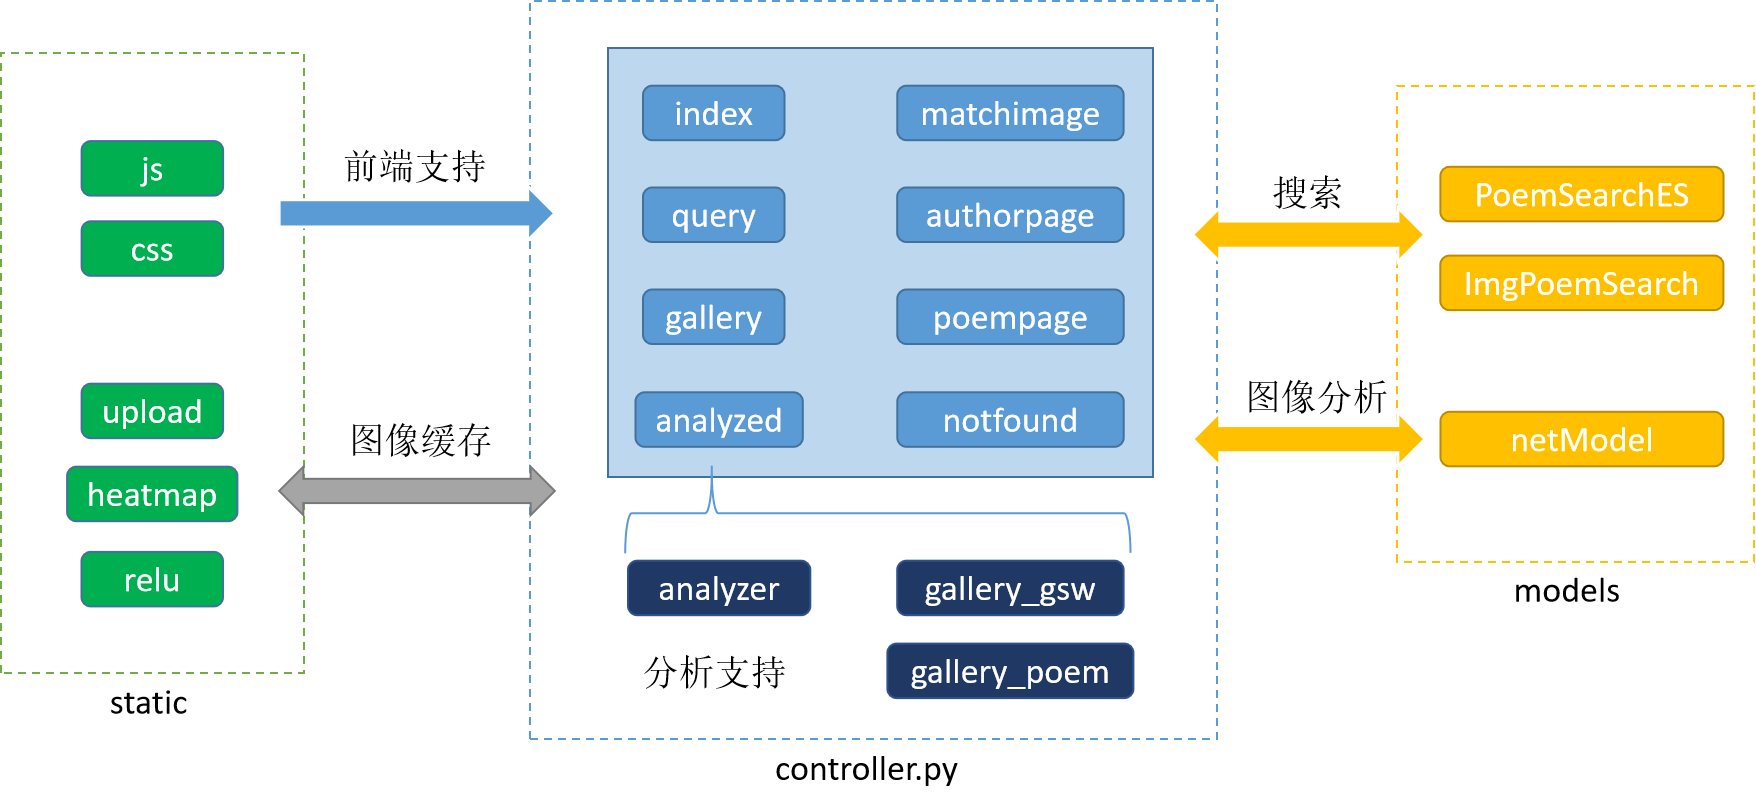
\includegraphics[scale=0.48]{fig/web_struct.png}
\caption{网站架构}
\label{fig:web_struct}
\end{figure}

图\ref{fig:web_struct}是我们搜索引擎的网站架构。

我们的网站采用了一定的MVC分离。PoemSeachES和netModel及model文件夹下的模型为搜索引擎的模型部分,负责对controller发出的查询请求做出响应和进行图像处理。controller.py为我们的控制器,图中由淡蓝色矩形框出的类都有对应的前端页面,深蓝色标出的三个类通过前端的javascript进行动态加载,异步返回数据。static是web.py框架下网站的资源文件夹,其中的js文件夹和css文件夹包含了支持前端布局的js文件和css文件,其余三个文件夹用于缓存用户上传和图像处理中间结果的图片。

\begin{table}[H]
\centering
\begin{tabular}{ccc}
\hline
\textbf{类} & \textbf{URL} & \textbf{页面} \\ \hline
index & /index & 首页推荐 \\
query & /query & 文本和图像查询处理结果页面,无翻页功能 \\ 
gallery & /gallery & 同query,但只处理文本查询,提供翻页接口 \\ 
poempage & /poempage & 单首诗歌内容页面 \\ 
authorpage & /authorpage & 单个作者信息及作品页面 \\ 
matchimage & /matchimage & 诗歌配图页面 \\ 
analyzed & /analyzed & 图像分析页面 \\ 
notfound & /notfound & 404页面 \\ \hline
\end{tabular}
\caption{链接对应关系}
\label{tab:url_connect}
\end{table}

controller中各个类对应的url及前端页面功能如表\ref{tab:url_connect}所示。

在controller.py中,我们还有一系列辅助函数存放在validator类下,用来进行表单验证和表格输入的预处理。其中最主要的两个函数是form\_validate和to\_command\_dict。

form\_validate对于用户通过表单的输入进行验证并返回验证结果供调用者进一步判断页面的跳转。该函数会判断用户的输入是否为空,其会检查所有可能成为有效输入的域,包括高级搜索中的精确搜索域。该函数还会检查表单输入的合法性,来避免用户的恶意访问。两个关键的准则是表单中包含searchType和query这两个域,因为他们确定了查询的索引和查询的内容(虽然query可以为空),和存在query模糊查询时高级搜索中的搜索域选择非空,否则这条查询无法转化成模型可以处理的命令。对于其他只应该由我们规定的内链所引起的查询,我们或者重用了form\_validate,或者实现了各自的验证函数来保证没有会造成严重后果的恶意访问发生。

to\_command\_dict根据表单提供的不同的查询约束,生成对应的查询域和查询值的映射并规定每一条约束是否为强制的(精确查询的)。这个函数的意义在于实现搜索引擎建立与数据库建立、控制器与模型的解耦,避免了在多个文件中修改关键字名称的工作。

\subsection{索引搜索}

\end{document}